\documentclass{article}
\usepackage{amsmath, amsfonts, amssymb}
\usepackage[margin=0.5in]{geometry}
\usepackage{graphicx}
\graphicspath{ {images/} }

\setlength{\parskip}{\baselineskip}%
\setlength{\parindent}{0pt}%

\title{Homework 3}
\author{Daniel Hartig}


\begin{document}
\maketitle

\subsubsection*{e. 2.}
For the ridge regression function $$\left|\mathbf{y}_{\text{train}}-\mathbf{\Phi}_{\text{train}}w\right|^2_2 + \lambda\left|w\right|^2_2,$$ then we can solve for a minimum by taking the zeroes of the derivative. 
\begin{align*}
\frac{d}{dw}\left(\left|\mathbf{y}_{\text{train}}-\mathbf{\Phi}_{\text{train}}w\right|^2_2 + \lambda\left|w\right|^2_2\right) &= -2\mathbf{\Phi}_{\text{train}}^\intercal\left(\mathbf{y_{\text{train}}} - \mathbf{\Phi}w\right)+2\lambda w = 0 \\
-2\mathbf{\Phi}_{\text{train}}^\intercal\mathbf{\Phi}_{\text{train}}w - 2\lambda w &= -2\mathbf{\Phi}_{\text{train}}^\intercal\mathbf{y_{\text{train}}} \\
w &= \left(\mathbf{\Phi}_{\text{train}}^\intercal\mathbf{\Phi}_{\text{train}} + \lambda \mathbf{I}_{D}\right)^{-1}\mathbf{\Phi}_{\text{train}}^\intercal\mathbf{y}_{\text{train}}
 \end{align*}
 
Using the singular value decomposition of $\mathbf{\Phi} = \mathbf{U}\mathbf{S}\mathbf{V}^\intercal$, and the spectral decomposition
\begin{align*}
\mathbf{\Phi}\mathbf{\Phi}^\intercal &= \left(\mathbf{U}\mathbf{S}\mathbf{V}^\intercal\right)\left(\mathbf{U}\mathbf{S}\mathbf{V}^\intercal\right)^\intercal \\
&=\mathbf{V}\mathbf{S}^\intercal\mathbf{U}^\intercal\mathbf{U}\mathbf{S}\mathbf{V}^\intercal \\
&=\mathbf{V}\mathbf{S}^2\mathbf{V}^\intercal
\end{align*}

Plugging this into the formula for $w$ gives, and utilizing the property that the transpose of a square diagonal matrix is itself ($\mathbf{S}^\intercal = \mathbf{S}$),
\begin{align*}
w &= \left(\mathbf{V}\mathbf{S}^2\mathbf{V}^\intercal + \lambda\mathbf{I}_D\right)\left(\mathbf{U}\mathbf{S}\mathbf{V}^\intercal\right)^\intercal\mathbf{y}_{\text{train}} \\
&=\mathbf{V}\left(\mathbf{S}^2+ \lambda\mathbf{I}_D\right)\mathbf{V}^\intercal\mathbf{V}\mathbf{S}^\intercal\mathbf{U}^\intercal\mathbf{y}_{\text{train}} \\
& = \mathbf{V}\left(\mathbf{S}^2+ \lambda\mathbf{I}_D\right)\mathbf{S}\mathbf{U}^\intercal\mathbf{y}_{\text{train}}
\end{align*}

$\left(\mathbf{S}^2+ \lambda\mathbf{I}_D\right)\mathbf{S}$ resolves to a diagonal matrix whose trace is 
\[\text{tr}\left(\mathbf{S}_\lambda\right) = \sum_{j=1}^{D} \frac{d_j}{d_j^2+\lambda}\] yielding the final form \[\mathbf{V}\mathbf{S}_\lambda\mathbf{U}^\intercal\mathbf{y}_{\text{train}}.\]

\subsubsection*{e. 3.}

The computational complexity of multplying an $n\times m$ matrix by an $m\times p$ matrix is $O(nmp)$. Multiplying $S_\lambda$ (a $D\times D$ matrix) by $\mathbf{U}^\intercal$ ($D\times n$) has a complexity of $O(nD^2)$ flops.

However, if we pre-compute $\mathbf{U}^\intercal\mathbf{y}_{\text{train}}$ only one time, then each matrix multiplication operation in the loop is $(D\times D)\times(D\times1)$; by multiplying  $\mathbf{U}^\intercal\mathbf{y}_{\text{train}}$ first by $S_\lambda$ then by $\mathbf{V}$. These operations have a complexity of $O(D^2)$ flops.

\pagebreak
\subsubsection*{i.)}

The test errors for both methods combined are:

\begin{center}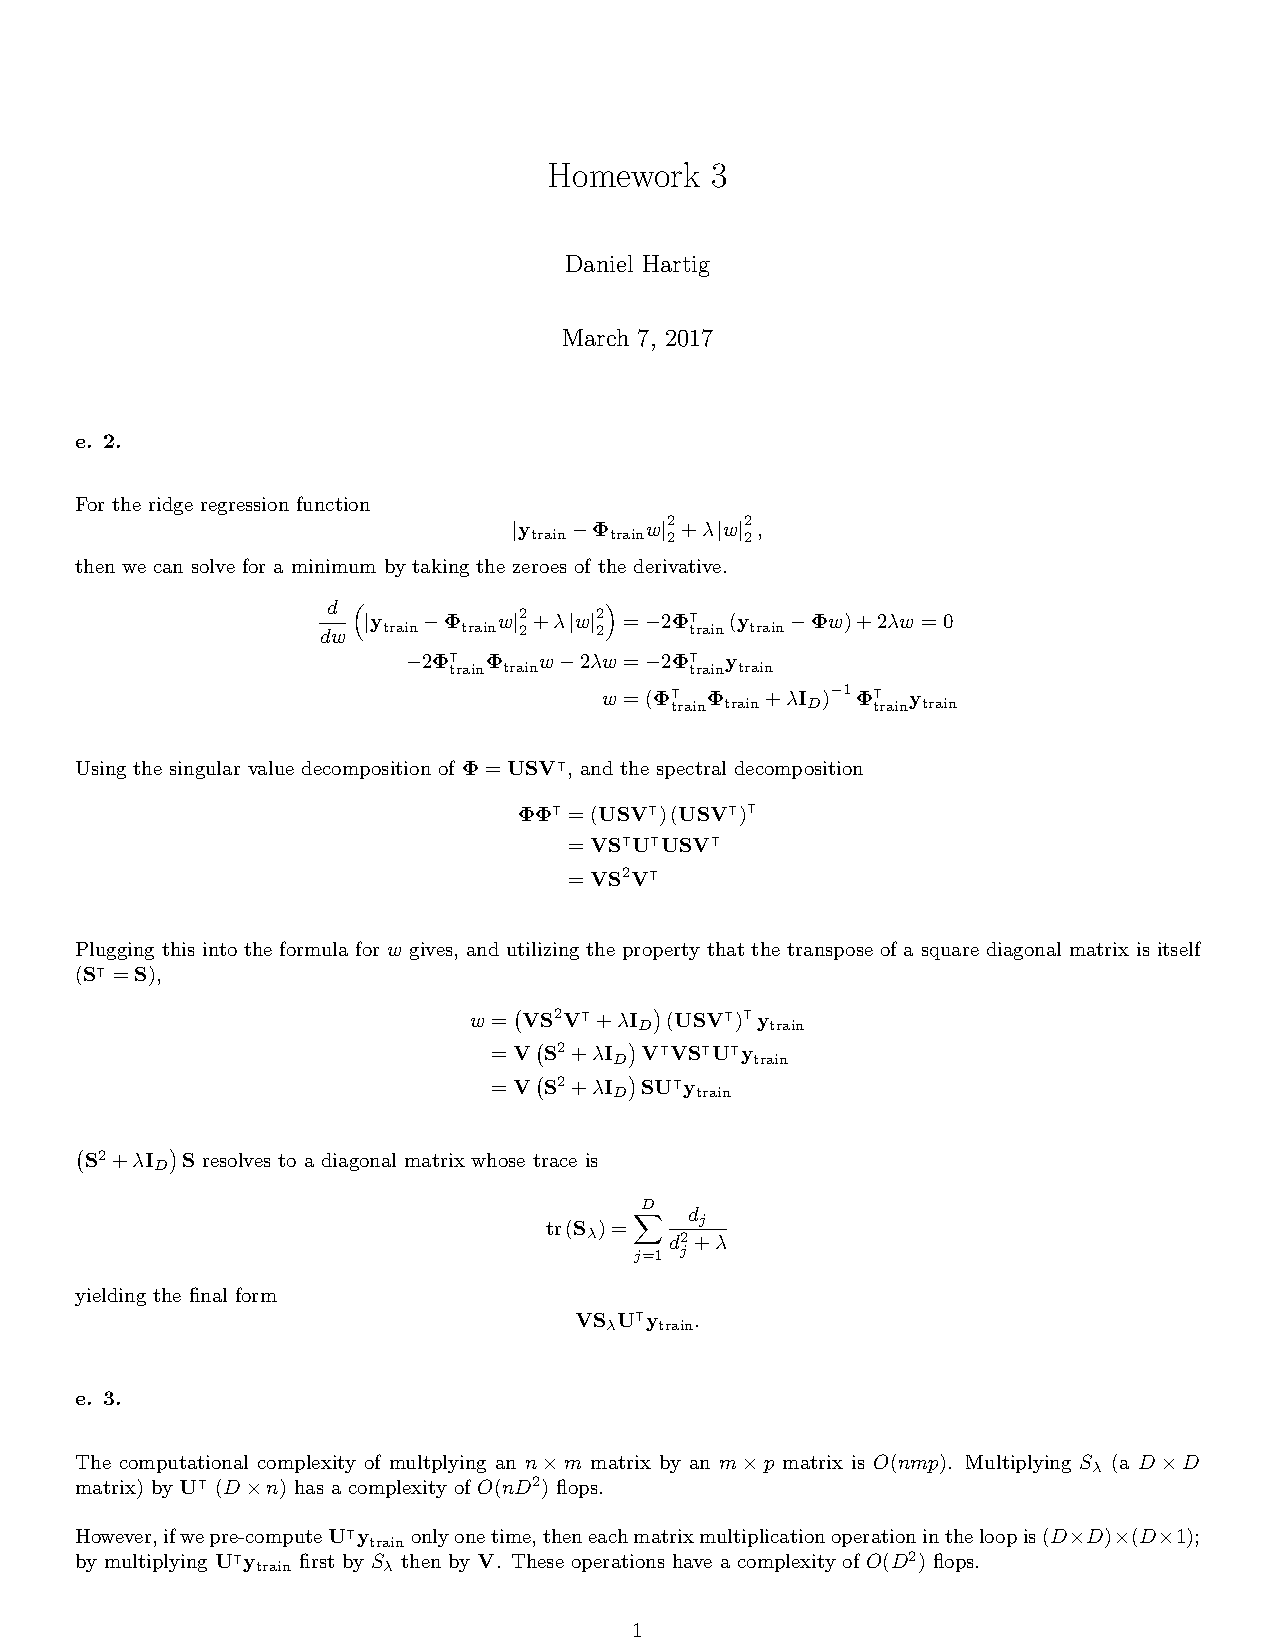
\includegraphics[scale=0.8]{hw3}\end{center}

We can see from the graphs that both methods converge to a similar error rate as $\lambda$ increases, but that Lasso regression holds that low error rate over a wider range of lambda values. Lasso regression also has a lower error rate at low values of lambda. Lasso regresion holds the lowest error rate of $0.072$ when $\lambda = \sqrt{\frac{\log D}{n_{\text{train}}}}2^{-6}$

\end{document}
